% Options for packages loaded elsewhere
\PassOptionsToPackage{unicode}{hyperref}
\PassOptionsToPackage{hyphens}{url}
\documentclass[
]{article}
\usepackage{xcolor}
\usepackage{amsmath,amssymb}
\setcounter{secnumdepth}{-\maxdimen} % remove section numbering
\usepackage{iftex}
\ifPDFTeX
  \usepackage[T1]{fontenc}
  \usepackage[utf8]{inputenc}
  \usepackage{textcomp} % provide euro and other symbols
\else % if luatex or xetex
  \usepackage{fontspec}
  \usepackage{unicode-math}
  \defaultfontfeatures{Scale=MatchLowercase}
  \defaultfontfeatures[\rmfamily]{Ligatures=TeX,Scale=1}
\fi
% Thai font support (XeLaTeX/LuaLaTeX)
\ifXeTeX
  \usepackage{xltxtra}
  \usepackage{polyglossia}
  \setmainlanguage{thai}
  \setotherlanguage{english}
  \setmainfont{TH Sarabun New}[
    BoldFont       = {TH Sarabun New Bold},
    ItalicFont     = {TH Sarabun New Italic},
    BoldItalicFont = {TH Sarabun New BoldItalic},
    Script         = Thai
  ]
\else\ifLuaTeX
  \usepackage{fontspec}
  \usepackage{polyglossia}
  \setmainlanguage{thai}
  \setotherlanguage{english}
  \setmainfont{TH Sarabun New}[
    BoldFont       = {TH Sarabun New Bold},
    ItalicFont     = {TH Sarabun New Italic},
    BoldItalicFont = {TH Sarabun New BoldItalic},
    Script         = Thai
  ]
\fi\fi
% Use upquote if available, for straight quotes in verbatim environments
\IfFileExists{upquote.sty}{\usepackage{upquote}}{}
\IfFileExists{microtype.sty}{% use microtype if available
  \usepackage[]{microtype}
  \UseMicrotypeSet[protrusion]{basicmath} % disable protrusion for tt fonts
}{}
\makeatletter
\@ifundefined{KOMAClassName}{% if non-KOMA class
  \IfFileExists{parskip.sty}{%
    \usepackage{parskip}
  }{% else
    \setlength{\parindent}{0pt}
    \setlength{\parskip}{6pt plus 2pt minus 1pt}}
}{% if KOMA class
  \KOMAoptions{parskip=half}}
\makeatother
\usepackage{longtable,booktabs,array}
\newcounter{none} % for unnumbered tables
\usepackage{multirow}
\usepackage{calc} % for calculating minipage widths
% Correct order of tables after \paragraph or \subparagraph
\usepackage{etoolbox}
\makeatletter
\patchcmd\longtable{\par}{\if@noskipsec\mbox{}\fi\par}{}{}
\makeatother
% Allow footnotes in longtable head/foot
\IfFileExists{footnotehyper.sty}{\usepackage{footnotehyper}}{\usepackage{footnote}}
\makesavenoteenv{longtable}
\usepackage{graphicx}
\makeatletter
\newsavebox\pandoc@box
\newcommand*\pandocbounded[1]{% scales image to fit in text height/width
  \sbox\pandoc@box{#1}%
  \Gscale@div\@tempa{\textheight}{\dimexpr\ht\pandoc@box+\dp\pandoc@box\relax}%
  \Gscale@div\@tempb{\linewidth}{\wd\pandoc@box}%
  \ifdim\@tempb\p@<\@tempa\p@\let\@tempa\@tempb\fi% select the smaller of both
  \ifdim\@tempa\p@<\p@\scalebox{\@tempa}{\usebox\pandoc@box}%
  \else\usebox{\pandoc@box}%
  \fi%
}
% Set default figure placement to htbp
\def\fps@figure{htbp}
\makeatother
\ifLuaTeX
  \usepackage{luacolor}
  \usepackage[soul]{lua-ul}
\else
  \usepackage{soul}
\fi
\setlength{\emergencystretch}{3em} % prevent overfull lines
\providecommand{\tightlist}{%
  \setlength{\itemsep}{0pt}\setlength{\parskip}{0pt}}
\usepackage{bookmark}
\IfFileExists{xurl.sty}{\usepackage{xurl}}{} % add URL line breaks if available
\urlstyle{same}
\hypersetup{
  hidelinks,
  pdfcreator={LaTeX via pandoc}}

\author{}
\date{}

\begin{document}

\textbf{แบบเสนอโครงการวิจัย}

\textbf{ประกอบการเสนอขอทุนสนับสนุนการวิจัย}

\textbf{จากกองทุนวิจัยมหาวิทยาลัยธรรมศาสตร์ ประจำปีงบประมาณ 2567}

\textbf{ประเภททุนวิจัยพัฒนาศักยภาพผลงานวิจัย (Fast Track)}

-\/-\/-\/-\/-\/-\/-\/-\/-\/-\/-\/-\/-\/-\/-\/-\/-\/-\/-\/-\/-\/-\/-\/-\/-\/-\/-\/-\/-\/-\/-\/-\/-\/-\/-\/-

ส่วนที่ 1 : รายละเอียดโครงการ

\subparagraph{ชื่อโครงการวิจัย (ภาษาไทย)
กรอบการเรียนรู้เชิงลึกแบบทั่วไปสำหรับการตรวจจับสิวด้วยชุดข้อมูลเปิดที่หลากหลาย}\label{uxe0auxe2duxe42uxe04uxe23uxe07uxe01uxe32uxe23uxe27uxe08uxe22-uxe20uxe32uxe29uxe32uxe44uxe17uxe22-uxe01uxe23uxe2duxe1auxe01uxe32uxe23uxe40uxe23uxe22uxe19uxe23uxe40uxe0auxe07uxe25uxe01uxe41uxe1auxe1auxe17uxe27uxe44uxe1buxe2auxe33uxe2buxe23uxe1auxe01uxe32uxe23uxe15uxe23uxe27uxe08uxe08uxe1auxe2auxe27uxe14uxe27uxe22uxe0auxe14uxe02uxe2duxe21uxe25uxe40uxe1buxe14uxe17uxe2buxe25uxe32uxe01uxe2buxe25uxe32uxe22}

\subparagraph{(ภาษาอังกฤษ) General Deep Learning Framework for Acne
Detection with Multiple Open
Datasets}\label{uxe20uxe32uxe29uxe32uxe2duxe07uxe01uxe24uxe29-general-deep-learning-framework-for-acne-detection-with-multiple-open-datasets}

\begin{enumerate}
\def\labelenumi{\arabic{enumi}.}
\setcounter{enumi}{1}
\item
  \textbf{คณะผู้วิจัย} (โปรดระบุประวัติของคณะผู้วิจัยทุกคนในข้อเสนอโครงการวิจัย ส่วนที่ 2)
\end{enumerate}

\begin{enumerate}
\def\labelenumi{\arabic{enumi}.}
\item
  \textbf{หัวหน้าโครงการวิจัย}
\end{enumerate}

\begin{quote}
ตำแหน่งทางวิชาการ ชื่อ-นามสกุล \ul{ผู้ช่วยศาสตราจารย์ ดร.กฤตคม ศรีจิรานนท์}

สังกัด \ul{คณะวิทยาศาสตร์และเทคโนโลยี ศูนย์ลำปาง} สัดส่วนในการทำวิจัย ร้อยละ \ul{75}
\end{quote}

\begin{enumerate}
\def\labelenumi{\arabic{enumi}.}
\setcounter{enumi}{1}
\item
  \textbf{ผู้ร่วมวิจัย}
\end{enumerate}

ตำแหน่งทางวิชาการ ชื่อ-นามสกุล \ul{รองศาสตราจารย์ ดร.ธนาธร ทะนานทอง}

สังกัด \ul{คณะวิทยาศาสตร์และเทคโนโลยี} สัดส่วนในการทำวิจัย ร้อยละ \ul{25}

\textbf{3. ที่ปรึกษาโครงการวิจัย} (ถ้ามี)

\begin{quote}
ตำแหน่งทางวิชาการ ชื่อ-นามสกุล

สังกัด
\end{quote}

\begin{enumerate}
\def\labelenumi{\arabic{enumi}.}
\setcounter{enumi}{2}
\item
  \textbf{ประเภทการวิจัย (เลือกข้อใดข้อหนึ่ง)}
\end{enumerate}

🔿 วิจัยพื้นฐาน

🔿 วิจัยประยุกต์

🔿 งานวิจัยเพื่อตอบปัญหาและพัฒนาชุมชน/สังคม

🔿 งานวิจัยเสริมหลักสูตรเพื่อพัฒนาการเรียนรู้ หลักสูตร/รหัสวิชา

🔿 อื่นๆ โปรดระบุ

\begin{enumerate}
\def\labelenumi{\arabic{enumi}.}
\setcounter{enumi}{3}
\item
  \textbf{สาขาที่สอดคล้องกับการวิจัย}
\end{enumerate}

\begin{quote}
🔿 \textbf{สาขาสังคมศาสตร์}

🔿 \textbf{สาขามนุษยศาสตร์}

🔿 \textbf{สาขาวิทยาศาสตร์และเทคโนโลยี}

🔿 \textbf{สาขาวิทยาศาสตร์สุขภาพ}
\end{quote}

\textbf{\hfill\break
5. ประเด็นการวิจัย มหาวิทยาลัยธรรมศาสตร์}

\textbf{เป้าหมายการพัฒนาที่ยั่งยืนตามแนวทางของสหประชาชาติ (Sustainable
Development Goals-SDGs) ใน 17 เป้าหมาย (Goals)}
(โปรดเลือกเป้าหมายที่โครงการของท่านเกี่ยวข้องมากที่สุด)

\textbf{□ เป้าหมายที่ 1} ยุติความยากจนทุกรูปแบบในทุกที่

\textbf{□ เป้าหมายที่ 2} ยุติความหิวโหย บรรลุความมั่นคงทางอาหารและยกระดับโภชนาการ
และส่งเสริมเกษตรกรรมที่ยั่งยืน

\textbf{□ เป้าหมายที่ 3}
สร้างหลักประกันว่าคนมีชีวิตที่มีสุขภาพดีและส่งเสริมสวัสดิภาพสำหรับทุกคน\\
ในทุกวัย

\textbf{□ เป้าหมายที่ 4}
สร้างหลักประกันว่าทุกคนมีการศึกษาที่มีคุณภาพอย่างครอบคลุมและเท่าเทียม
และสนับสนุนโอกาสในการเรียนรู้ตลอดชีวิต

\textbf{□ เป้าหมายที่ 5} บรรลุความเท่าเทียมระหว่างเพศ
และเสริมสร้างความเข้มแข็งให้แก่สตรีและเด็กหญิง

\textbf{□ เป้าหมายที่ 6} สร้างหลักประกันเรื่องน้ำและการสุขาภิบาลให้มีการจัดการอย่างยั่งยืน
และมีสภาพพร้อมใช้สำหรับทุกคน

\textbf{□ เป้าหมายที่ 7}
สร้างหลักประกันให้ทุกคนสามารถเข้าถึงพลังงานสมัยใหม่ที่ยั่งยืนในราคา\\
ที่ย่อมเยา

\textbf{□ เป้าหมายที่ 8} ส่งเสริมการเติบโตทางเศรษฐกิจที่ต่อเนื่อง ครอบคลุมและยั่งยืน
การจ้างงานเต็มที่ และการมีงานที่สมควรสำหรับทุกคน

\textbf{□ เป้าหมายที่ 9} สร้างโครงสร้างพื้นฐานที่มีความทนทาน
ส่งเสริมการพัฒนาอุตสาหกรรม\\
ที่ครอบคลุมและยั่งยืน และส่งเสริมนวัตกรรม

\textbf{🗹 เป้าหมายที่ 10} ลดความไม่เสมอภาคภายในประเทศและระหว่างประเทศ

\textbf{□ เป้าหมายที่ 11} ทำให้เมืองและการตั้งถิ่นฐานของมนุษย์มีความปลอดภัย ทั่วถึง
พร้อมรับการเปลี่ยนแปลงและยั่งยืน

\textbf{□ เป้าหมายที่ 12} สร้างหลักประกันให้มีรูปแบบการผลิตและการบริโภคที่ยั่งยืน

\textbf{□ เป้าหมายที่ 13}
ปฏิบัติการอย่างเร่งด่วนเพื่อต่อสู้กับการเปลี่ยนแปลงสภาพภูมิอากาศและผลกระทบที่เกิดขึ้น

\textbf{□ เป้าหมายที่ 14} อนุรักษ์และใช้ประโยชน์จากมหาสมุทร ทะเล
และทรัพยากรทางทะเลอย่างยั่งยืน เพื่อการพัฒนาที่ยั่งยืน

\textbf{□ เป้าหมายที่ 15} ปกป้อง ฟื้นฟู และสนับสนุนการใช้ระบบนิเวศบนบกอย่างยั่งยืน
จัดการป่าไม้อย่างยั่งยืน ต่อสู้การกลายสภาพเป็นทะเลทราย หยุดการเสื่อมโทรมของที่ดิน
และฟื้นสภาพกลับมาใหม่ และหยุดการสูญเสียความหลากหลายทางชีวภาพ

\textbf{□ เป้าหมายที่ 16} ส่งเสริมสังคมที่สงบสุขและครอบคลุมเพื่อการพัฒนาที่ยั่งยืน
ให้ทุกคนเข้าถึงความยุติธรรมและสร้างสถาบันที่มีประสิทธิผลรับผิดชอบและครอบคลุมในทุกระดับ

\textbf{□ เป้าหมายที่ 17}
เสริมความเข้มแข็งให้แก่กลไกการดำเนินงานและฟื้นฟูสภาพหุ้นส่วน\\
ความร่วมมือระดับโลกสำหรับการพัฒนาที่ยั่งยืน

* โดยนักวิจัยสามารถศึกษา ข้อมูลที่เกี่ยวกับ SDGs ศึกษาได้จาก
\url{https://sdgs.tu.ac.th}

\textbf{6. โปรดระบุความเกี่ยวข้องกับมาตรฐานการทำวิจัย} (ทำเครื่องหมาย ✔ ในช่อง 🔿
พร้อมแนบเอกสาร)

\begin{quote}
\textbf{6.1} 🔿 \textbf{จริยธรรมการวิจัยในคน}

\textbf{6.2 🔿 การใช้สัตว์ทดลอง}

\textbf{6.3 🔿 การดำเนินการด้านความปลอดภัยทางชีวภาพ}

\textbf{6.4 🔿 โครงการนี้ไม่เกี่ยวข้อง}
\end{quote}

\textbf{หมายเหตุ} 1) หากระบุความเกี่ยวข้องตามข้อ 6.1 -- 6.3
ต้องแนบหลักฐานการผ่านการรับรองจากคณะกรรมการ พร้อมกับการยื่นข้อเสนอโครงการวิจัย

2) หากระบุว่าไม่เกี่ยวข้องและมีผลสืบเนื่องในเรื่องที่เกี่ยวข้องกับมาตรฐานการทำวิจัยในภายหลัง
จะไม่เป็นความรับผิดชอบของมหาวิทยาลัย และจะถือว่าเป็นความรับผิดชอบของคณะผู้วิจัยเท่านั้น

\textbf{7. คำสำคัญ (keyword)}

คำสำคัญ (ภาษาไทย) โครงข่ายประสาทเทียมแบบคอนโวลูชัน, การตรวจจับสิว,

การจำแนกระดับความรุนแรง, การเรียนรู้เชิงลึก, ปัญญาประดิษฐ์

คำสำคัญ (ภาษาอังกฤษ) Convolutional neural networks, Acne detection,\\
Severity grading classification, Deep learning,

Artificial intelligence

\textbf{8. ความสำคัญและที่มาของปัญหาที่ทำการวิจัย/ความสอดคล้องกับยุทธศาสตร์}

Acne is one of the most ubiquitous skin diseases that occur on 90\% of
human population {[}1{]}, and it is most common in adolescents and
adults. Acne manifests in various forms, including whiteheads (closed
plugged pores), blackheads (open plugged pores), small red tender bumps
(papules), pimples (pustules), large solid painful lumps under the skin
(nodules), and painful pus-filled lumps under the skin (cystic lesions).
These lesions commonly appear on the face, chest, shoulders, and upper
back {[}2{]}. There are many negative effects of acne, such as
significant skin damage and a negative impact on a
patient\textquotesingle s mental health, which can lead to reduced
self-esteem, particularly among adolescents {[}3{]}. The diagnosis of
acne involves grading severity levels by counting the number of acne
lesions based on various criteria, such as the Hayashi Criteria {[}4{]}
and the Global Acne Grading System (GAGS) {[}5{]}. Currently, the
prevailing method for diagnosing the acne severity is manually count the
acne by dermatologists. However, this method is time-consuming and prone
to errors, resulting in potential misdiagnosis.

In recent years, there have been substantial improvements in Artificial
Intelligence (AI), leading to its integration across various fields,
particularly in the healthcare industry. AI is utilized for a wide range
of applications, including using AI in Raman spectroscopy for diagnosing
tumors {[}6{]}, detecting glaucoma from images {[}7{]}, and applying AI
with initial chest X-ray and electronic health record data to predict
the prognosis or mortality of COVID-19 {[}8{]}. The background of AI in
object detection and identification lies in machine learning,
particularly deep learning. Several studies have implemented deep
learning models for acne detection and severity grading for helping
individuals who do not have access to dermatologists in diagnosing the
severity of an acne and streamline the process for dermatologists. For
example, regression models and Faster Region-based Convolutional Neural
Networks (Faster-RCNN) are utilized to grade acne severity on ACNE04
dataset {[}9{]}. Modified Pyramid Scene Parsing Network (PSPNet)
proposed by {[}10{]} is utilized to grade acne severity on their own
private dataset from Xiangya Hospital to create model. However, much of
the research has focused on training models with only one specific
dataset and fine-tuning them until optimal accuracy is achieved. There
are only a few studies, such as the research conducted by {[}11{]}, that
applied Diagnostic Evidence Distillation (DED), which is based on
Convolutional Neural Networks (CNNs), to grade acne severity on ACNE04
and PLSBRACNE01 datasets. This research achieved precision and accuracy
of 86.06\% and 85.31\% on the ACNE04 dataset, and 69.16\% and 67.56\% on
the PLSBRACNE01 dataset, respectively. These results show a significant
drop in precision and accuracy from the ACNE04 dataset to the
PLSBRACNE01 dataset by 16.9\% and 17.75\%, respectively.

This research proposes a novel deep learning model for acne detection
and severity grading classification by extending popular deep learning
models with CNN-based architectures as backbones. Additionally, the
proposed model utilizes multiple open datasets to train and optimize its
performance. The primary objective of this study is to achieve superior
performance across diverse datasets and compare the
model\textquotesingle s effectiveness with previous research studies.
Furthermore, this research introduces a framework and publishes
application programming interfaces (APIs) that empower other researchers
and developers to enhance the framework\textquotesingle s
functionalities or build upon it. The offered APIs are easily adoptable
and applicable in real-world applications. Moreover, these APIs serve
valuable educational purposes, allowing students and researchers to
explore the inner workings of the framework and gain insights from its
design choices.

\textbf{9. วัตถุประสงค์ของโครงการ}

\begin{itemize}
\item
  To design and implement a deep learning model with CNN-based
  architectures as backbones for acne detection and severity grading
  classification that utilizes multiple standard datasets, aiming to
  achieve superior performance across various data samples.
\item
  To develop a knowledge-based framework using the proposed model by
  creating an Application Programming Interface (API) that allows users
  to request application development.
\end{itemize}

\textbf{10. ขอบเขตของโครงการ}

\begin{itemize}
\item
  Develop a deep learning model with CNN-based architectures as
  backbones for acne detection and severity grading classification,
  capable of detecting and classifying images.
\item
  Select and utilize various standard open datasets to train and
  validate the model.
\item
  Improve the accuracy and efficiency of the proposed deep learning
  model through optimization techniques and algorithm enhancements.
\item
  Create a knowledge-based framework for acne detection and severity
  grading classification that can be applied to diverse applications and
  scenarios.
\end{itemize}

\textbf{11. ทฤษฎี สมมุติฐาน (ถ้ามี) และกรอบแนวคิดของโครงการ}

11.1 Image Processing

Image processing stands as one of the most prevalent techniques employed
to enhance accuracy in deep learning models. This technique encompasses
a variety of methods, including converting images to grayscale,
eliminating backgrounds, and employing augmentation. For instance, in
the study {[}12{]}, the implementation comprised face detection using
Baidu AI\textquotesingle s SDK, attention extraction for segmenting face
pixels, and image augmentation, culminating in an accuracy of 84.52\% on
the ACNE04 dataset and 52.85\% on the PLSBRACNE01 dataset. In another
research endeavor {[}13{]}, gray-scale conversion, face detection using
Haar Cascade Classifier, background removal using GrabCut, and
heat-mapping were harnessed for image processing, yielding a
sensitivity, precision, and accuracy of 78\%, 90\%, and 73\%,
correspondingly, on their private dataset.

However, numerous studies achieve remarkable outcomes without the
application of any image processing techniques. For instance, in the
study {[}14{]}, ResNet-50 served as a backbone, attaining an accuracy of
84.11\% on the ACNE04 dataset sans any image processing. Similarly, in
the research {[}15{]}, Faster-RCNN was enlisted as the backbone,
achieving an accuracy of 85\% on their private dataset devoid of image
processing. Therefore, this study aims to incorporate experiments
involving image processing to enhance the performance of the proposed
deep learning model.

11.2 Object Detection with Deep Learning Model

Deep learning constitutes a subset of machine learning, essentially
representing a neural network with three or more layers designed to
simulate the human brain\textquotesingle s functionality. This design
enables it to grasp insights from a vast amount of data. Deep learning
finds application in various tasks, including voice recognition, text
generation, and object detection. Notably, convolutional neural networks
(CNNs) stand as one of the most prominent types of deep learning,
particularly deployed for image recognition and computer vision tasks.
CNNs eliminate the need for manual feature extraction by directly
discerning features from images. This inherent feature extraction
capability allows deep learning to excel in computer vision endeavors,
resulting in high accuracy, particularly in object detection.

Several deep learning architectures incorporate CNN as a backbone:

\begin{itemize}
\item
  VGG16 {[}16{]}, a CNN-based architecture boasting 16 layers and
  employing large kernel-sized filters, often using multiple (3x3)
  kernel-sized filters consecutively.
\item
  ResNet {[}17{]}, a solution addressing the issue of error rate
  escalation when deepening networks, primarily tackling the Vanishing
  Gradient problem inherent in deep learning.
\item
  YOLO {[}18{]}, one of the most popular deep learning models for object
  detection, is also rooted in CNN. The YOLO algorithm stands out for
  requiring just one forward propagation, enabling it to predict an
  entire image in a single algorithmic run.
\item
  Faster R-CNN {[}19{]} stands as a deep learning architecture building
  upon the Fast R-CNN framework. It enhances the original CNN-based Fast
  R-CNN by incorporating a region proposal network (RPN). The
  integration of RPN with Fast R-CNN results in a unified network that
  shares convolutional features between these two constituent
  components.
\end{itemize}

\textbf{12. การทบทวนวรรณกรรม/สารสนเทศ (information) ที่เกี่ยวข้อง}

12.1 Open-sources datasets for acne

The datasets are collected by searching for open datasets from popular
sources such as Kaggle and Roboflow, as well as possibly requesting
access to private data from researchers. The collected open dataset
consists of six popular datasets selected from a variety of researchers,
with the details shown in Table 1.

Table 1 A summary of the preliminary open dataset

{\def\LTcaptype{none} % do not increment counter
\begin{longtable}[]{@{}
  >{\raggedright\arraybackslash}p{(\linewidth - 4\tabcolsep) * \real{0.2037}}
  >{\raggedright\arraybackslash}p{(\linewidth - 4\tabcolsep) * \real{0.1630}}
  >{\raggedright\arraybackslash}p{(\linewidth - 4\tabcolsep) * \real{0.6332}}@{}}
\toprule\noalign{}
\begin{minipage}[b]{\linewidth}\centering
\textbf{Dataset name}
\end{minipage} & \begin{minipage}[b]{\linewidth}\centering
\textbf{The number of images}
\end{minipage} & \begin{minipage}[b]{\linewidth}\centering
\textbf{Details}
\end{minipage} \\
\midrule\noalign{}
\endhead
\bottomrule\noalign{}
\endlastfoot
20 Skin Diseases Dataset {[}20{]} & 841 & This dataset includes 20 skin
diseases with 841 acne images \\
Skin Diseases {[}21{]} & 2150 & This dataset includes 6 skin diseases
with 2150 acne images \\
Dermnet {[}22{]} & 841 & This dataset includes 23 skin diseases with 841
acne images \\
Acne Grading Classification dataset {[}23{]} & 999 & This dataset
includes only acne images \\
Acne dataset {[}24{]} & 1834 & This dataset includes only acne images \\
ACNE04 {[}25{]} & 1419 & This dataset includes only acne images with
labels \\
\end{longtable}
}

12.2 Severity grading criteria

Severity grading criteria are used to assess the severity of acne, and
there are numerous such criteria, which can vary across different
studies. Each criterion differs in terms of the number of levels and the
quantity of acne in each level. Two prominent severity grading criteria
are the Hayashi Grading Criteria {[}4{]} and the Global Acne Grading
System Score (GAGS) {[}5{]}, and their details are provided in Table 2.

Table 2 International severity grading criteria

{\def\LTcaptype{none} % do not increment counter
\begin{longtable}[]{@{}
  >{\raggedright\arraybackslash}p{(\linewidth - 4\tabcolsep) * \real{0.1210}}
  >{\centering\arraybackslash}p{(\linewidth - 4\tabcolsep) * \real{0.3882}}
  >{\raggedright\arraybackslash}p{(\linewidth - 4\tabcolsep) * \real{0.1879}}@{}}
\toprule\noalign{}
\begin{minipage}[b]{\linewidth}\centering
\textbf{Criteria}
\end{minipage} & \begin{minipage}[b]{\linewidth}\centering
\textbf{The number of acne lesions}
\end{minipage} & \begin{minipage}[b]{\linewidth}\centering
\textbf{Meaning}
\end{minipage} \\
\midrule\noalign{}
\endhead
\bottomrule\noalign{}
\endlastfoot
Hayashi & 0 - 5 & none \\
& 6 - 20 & moderate \\
& 21 - 50 & severe \\
& more than 50 & very severe \\
GAGS & 0 & none \\
& 1 - 18 & mild \\
& 19 - 30 & moderate \\
& 31 - 38 & severe \\
& more than 38 & very severe \\
\end{longtable}
}

12.3 Summary

From the previous study, the deep learning model can be divided into
three types. The first type is a fine-tuning the exist deep learning
architectures {[}26{]} -- {[}31{]}. For instance, in study {[}30{]},
selected Inception v3 for acne detection, achieving an accuracy of
89.39\% by fine tuning the parameter. The second type is a proposed
novel model by using the exist deep learning architectures as a backbone
{[}10{]} -- {[}12{]}, {[}14{]}, {[}32{]} -- {[}36{]}. For instance, in
study {[}35{]}, VGG16 was utilized as a backbone by adding skin patch,
yielding an accuracy of 84.52\% on the ACNE04 dataset and 52.85\% on
PLSBRACNE01. The last type is using ensemble model with combine more
than one exists deep learning architectures {[}9{]}, {[}15{]}, {[}37{]}
-- {[}39{]}. For instance, in study {[}38{]}, ResNet-50 and YOLOv5 were
employed to create a hybrid deep learning model, which fine tuning
process was applied to both. ResNet-50 for classification module and
YOLOv5 for localization module, resulting in a remarkable accuracy of
99.31\% on the ACNE04 dataset.

The conclusions drawn from the details of the 20 selected articles are
summarized in Table 3, which includes the source of the dataset,
severity grading criteria, image processing techniques, deep learning
models employed, statistical indicators, and the model\textquotesingle s
outcomes. The key points are as follows:

\begin{itemize}
\item
  The collective findings of the studies reveal that 15 of them utilized
  open datasets, with 80\% of those studies employing the ACNE04
  dataset. This highlights the prevalence of ACNE04 as the most commonly
  adopted open dataset for acne severity grading.
\item
  Notably, only four articles incorporated more than one dataset, and
  their outcomes clearly illustrate a significant accuracy drop on the
  second dataset. For instance, in study {[}11{]}, DED was proposed,
  utilizing CNNs as a backbone for grading acne severity. The precision
  and accuracy achieved were 86.06\% and 85.31\% on the ACNE04 dataset,
  respectively, but decreased to 69.16\% and 67.56\% on the PLSBRACNE01
  dataset. Similarly, in {[}33{]}, Prior Knowledge Guided (PKG) was
  employed, using CNN as a backbone, resulting in an accuracy of 85.27\%
  on the ACNE04 dataset, but dropping to 65.85\% on the PLSBRACNE01
  dataset.
\item
  All the studies consistently utilized CNN-based models as the
  backbone.
\item
  Notably, one study introduced an open-source framework. In study
  {[}27{]}, ResNet served as the backbone for acne severity grading,
  yielding an RMSE of 0.78. However, the focus was limited to the
  forehead, right cheek, left cheek, and chin. In comparison with other
  studies, this model\textquotesingle s performance was comparatively
  lower.
\end{itemize}

Table 3 A summary of the previous studies in acne detection and severity
grading classification

{\def\LTcaptype{none} % do not increment counter
\begin{longtable}[]{@{}
  >{\raggedright\arraybackslash}p{(\linewidth - 12\tabcolsep) * \real{0.1757}}
  >{\raggedright\arraybackslash}p{(\linewidth - 12\tabcolsep) * \real{0.1362}}
  >{\raggedright\arraybackslash}p{(\linewidth - 12\tabcolsep) * \real{0.0646}}
  >{\raggedright\arraybackslash}p{(\linewidth - 12\tabcolsep) * \real{0.1816}}
  >{\raggedright\arraybackslash}p{(\linewidth - 12\tabcolsep) * \real{0.2424}}
  >{\raggedright\arraybackslash}p{(\linewidth - 12\tabcolsep) * \real{0.1062}}
  >{\raggedright\arraybackslash}p{(\linewidth - 12\tabcolsep) * \real{0.0934}}@{}}
\toprule\noalign{}
\begin{minipage}[b]{\linewidth}\centering
\textbf{Authors}
\end{minipage} & \begin{minipage}[b]{\linewidth}\centering
\textbf{Dataset}
\end{minipage} & \begin{minipage}[b]{\linewidth}\centering
\textbf{SGC}
\end{minipage} & \begin{minipage}[b]{\linewidth}\centering
\textbf{Image processing}
\end{minipage} & \begin{minipage}[b]{\linewidth}\centering
\textbf{Deep learning model}
\end{minipage} & \begin{minipage}[b]{\linewidth}\centering
\textbf{Statistical indicators}
\end{minipage} & \begin{minipage}[b]{\linewidth}\centering
\textbf{Outcomes}
\end{minipage} \\
\midrule\noalign{}
\endhead
\bottomrule\noalign{}
\endlastfoot
S. Alzahrani et al. {[}9{]} & ACNE04 & Hayashi & - & UNet dense
regressor and Faster R-CNN & MAE MSE Prec Spec Sens Acc & ASGC \\
J. Wang et al. {[}10{]} & Private dataset & GAGS & Background removal &
Localization-DL based on PSPNet and ClassSeg based on HRNet & Acc &
ASGC \\
Y. Lin et al. {[}11{]} & ACNE04 and PLSBRACNE01 & Hayashi & - & DED with
EfficientNet-based & Acc Prec Sens Spec YI & ASGC \\
Y. Lin et al. {[}12{]} & ACNE04 and PLSBRACNE01 & Hayashi & AES & SFNet
with VGG16-based & Acc & ASGC \\
X. Wu et al. {[}14{]} & ACNE04 & Hayashi & - & LDL and ResNet-50-based &
Acc & ASGC \\
Q. T. Huynh et al. {[}15{]} & Private Dataset & GEA & - & Faster R-CNN
and LightGBM & Acc & ASGC \\
N. Yadav et al. {[}26{]} & DermNet & - & k-mean, Gaussian method, and
HSV segmentation & CNN & Acc & AS \\
T. Zhao et al. {[}27{]} & Private dataset & Hayashi & Extracted and
Rolling skin patches & ResNet & RMSE & ASGC \\
A. R. Prodeep et al {[}28{]} & DermNet and AGC & - & - & EfficientNet &
Acc Prec Rec & AD \\
H. Zein et al. {[}29{]} & ACNE04 & Hayashi & - & InceptionResNetv2 & Acc
& ASGC \\
K. Naidu et al. {[}30{]} & DermNet & - & Background removal & Inception
V3 & Acc & AD \\
K. Rashataprucksa et al. {[}31{]} & Private Dataset & - & - & R-FCN &
Acc Prec AP & AD \\
M. S. Junayed et al. {[}32{]} & Private dataset & - & Contrast
Enhancement and Color Conversion & ScarNet with CNN-based & Acc Spec

KS & AD \\
Y. Lin et al. {[}33{]} & ACNE04 and PLSBRACNE01 & Hayashi & - & PKG with
CNN-based & Acc & ASGC \\
K. Min et al. {[}34{]} & ACNE04 & - & - & ACNet with CNN-based & mAP &
AD \\
Y. Lin et al. {[}35{]} & ACNE04 and PLSBRACNE01 & Hayashi & Information
Fold, Key area segmentation & GLFN with VGG16-based & Acc Sen Spec YI &
ASGC \\
X. Wei et al. {[}36{]} & Private Dataset

and ACNE04 & - & - & DSDH with Mask R-CNN-based & AP & AD \\
H. Wen et al. {[}37{]} & ACNE04 & Hayashi & - & R-CNN and YOLOv4 & mAP &
ASGC \\
H. Zhang et al. {[}38{]} & ACNE04 & Hayashi & - & ResNet50 and YOLOv5 &
Acc & ASGC \\
J. Zhang et al. {[}39{]} & Private Dataset and ACNE04 & - & - & SADH
with Mask R-CNN and ResNet50-based & AP & AD \\
\end{longtable}
}

Acc denotes accuracy, AD denotes acne detection, AES denotes attention
extraction segmentation AP denotes average precision, AS denotes acne
segmentation, ASGC denotes acne severity grading classification, DSDH
denotes Decoupled Sequential Detection Head, GEA denotes Global
Evaluation Acne, GLFN denotes Global local fusion network, KS denotes
Kappa Score, LDL denotes Label Distribution Learning, MAE denotes mean
absolute error, mAP denotes mean average precision, MSE denotes mean
squared error, Prec denotes precision, SADH denotes Spatial Aware Double
Head, Sens denotes sensitivity, SGC denotes severity grading criteria,
Spec denotes specificity, YI denotes Youden Index

\textbf{\hfill\break
13. วิธีการดำเนินการวิจัย (research methodology)}

13.1 The proposed framework

The process of the proposed framework, depicted in Figure 1, commences
with a user\textquotesingle s request for APIs and the submission of an
image intended for acne severity grading. Subsequently, the submitted
image undergoes assessment by a model that utilizes the novel deep
learning with CNN-based architectures as the backbone. This process
initiates with dataset collection, encompassing open datasets from
platforms like Kaggle and Roboflow, and potentially accessing private
data from researchers. The acquired dataset is meticulously prepared
using Extract, Transform, Load (ETL) techniques to ensure efficient data
storage. Diverse data preprocessing methods are then applied to
effectively clean the raw data. The subsequent phase involves creating a
novel deep learning model tailored for acne detection and severity
grading, potentially incorporating image processing techniques. This
stage encompasses exploring various combinations of deep learning
models, including, but not limited to, VGG16, ResNet, or other CNN-based
models, and proposing new techniques. The overarching goal is to
formulate an advanced and optimized model capable of accurately
discerning and categorizing distinct levels of acne severity. Finally,
the user receives the assigned severity level for the submitted image
based on the chosen grading criterion.

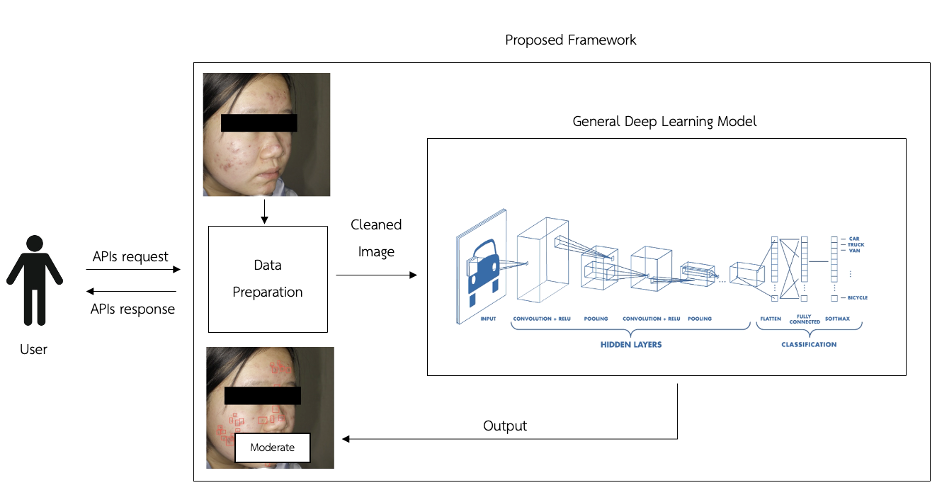
\includegraphics[width=6.50417in,height=3.40486in]{media/image1.png}

Figure 1 A process of the proposed AI framework

13.2 Experiments

Various experiments, incorporating hyperparameter tuning, are conducted
to identify and confirm the superior performance of the proposed deep
learning model. Additionally, models from previous research studies are
selected and implemented for comparison with the proposed model, using a
range of statistical indicators including average precision, mean
average precision, precision, sensitivity, specificity, and accuracy.

\textbf{14. ระยะเวลาการวิจัยทั้งโครงการ}
(นับจากระยะเวลาที่เริ่มต้นสัญญารับทุนไปจนถึงบทความได้รับการตอบรับให้ตีพิมพ์ในวารสารแล้ว)

ระยะเวลาโครงการ \ul{2} ปี \ul{0} เดือน

วันที่เริ่มต้น \ul{5 มิถุนายน 2567} วันที่สิ้นสุด \ul{4 มิถุนายน 2569}

\textbf{แผนการดำเนินงานวิจัย}

{\def\LTcaptype{none} % do not increment counter
\begin{longtable}[]{@{}
  >{\centering\arraybackslash}p{(\linewidth - 28\tabcolsep) * \real{0.0883}}
  >{\raggedright\arraybackslash}p{(\linewidth - 28\tabcolsep) * \real{0.2059}}
  >{\centering\arraybackslash}p{(\linewidth - 28\tabcolsep) * \real{0.0495}}
  >{\centering\arraybackslash}p{(\linewidth - 28\tabcolsep) * \real{0.0496}}
  >{\centering\arraybackslash}p{(\linewidth - 28\tabcolsep) * \real{0.0496}}
  >{\centering\arraybackslash}p{(\linewidth - 28\tabcolsep) * \real{0.0495}}
  >{\centering\arraybackslash}p{(\linewidth - 28\tabcolsep) * \real{0.0496}}
  >{\centering\arraybackslash}p{(\linewidth - 28\tabcolsep) * \real{0.0496}}
  >{\centering\arraybackslash}p{(\linewidth - 28\tabcolsep) * \real{0.0495}}
  >{\centering\arraybackslash}p{(\linewidth - 28\tabcolsep) * \real{0.0496}}
  >{\centering\arraybackslash}p{(\linewidth - 28\tabcolsep) * \real{0.0496}}
  >{\centering\arraybackslash}p{(\linewidth - 28\tabcolsep) * \real{0.0495}}
  >{\centering\arraybackslash}p{(\linewidth - 28\tabcolsep) * \real{0.0496}}
  >{\centering\arraybackslash}p{(\linewidth - 28\tabcolsep) * \real{0.0496}}
  >{\centering\arraybackslash}p{(\linewidth - 28\tabcolsep) * \real{0.1111}}@{}}
\toprule\noalign{}
\multirow{2}{=}{\centering\arraybackslash \begin{minipage}[b]{\linewidth}\centering
\textbf{ลำดับที่}
\end{minipage}} &
\multirow{2}{=}{\begin{minipage}[b]{\linewidth}\centering
\textbf{กิจกรรม}
\end{minipage}} &
\multicolumn{12}{>{\centering\arraybackslash}p{(\linewidth - 28\tabcolsep) * \real{0.5947} + 22\tabcolsep}}{%
\begin{minipage}[b]{\linewidth}\centering
\textbf{เดือนที่}
\end{minipage}} &
\multirow{2}{=}{\centering\arraybackslash \begin{minipage}[b]{\linewidth}\centering
\textbf{ร้อยละของกิจกรรม}
\end{minipage}} \\
& & \begin{minipage}[b]{\linewidth}\centering
\textbf{1}
\end{minipage} & \begin{minipage}[b]{\linewidth}\centering
\textbf{2}
\end{minipage} & \begin{minipage}[b]{\linewidth}\centering
\textbf{3}
\end{minipage} & \begin{minipage}[b]{\linewidth}\centering
\textbf{4}
\end{minipage} & \begin{minipage}[b]{\linewidth}\centering
\textbf{5}
\end{minipage} & \begin{minipage}[b]{\linewidth}\centering
\textbf{6}
\end{minipage} & \begin{minipage}[b]{\linewidth}\centering
\textbf{7}
\end{minipage} & \begin{minipage}[b]{\linewidth}\centering
\textbf{8}
\end{minipage} & \begin{minipage}[b]{\linewidth}\centering
\textbf{9}
\end{minipage} & \begin{minipage}[b]{\linewidth}\centering
\textbf{10}
\end{minipage} & \begin{minipage}[b]{\linewidth}\centering
\textbf{11}
\end{minipage} & \begin{minipage}[b]{\linewidth}\centering
\textbf{12}
\end{minipage} \\
\midrule\noalign{}
\endhead
\bottomrule\noalign{}
\endlastfoot
1 & Literature review & & & & & & & & & & & & & 5 \\
2 & Dataset collection & & & & & & & & & & & & & 5 \\
3 & Dataset preparation & & & & & & & & & & & & & 10 \\
4 & Designing and implementing a deep learning model with CNN-based
architectures as backbones & & & & & & & & & & & & & 30 \\
& & \textbf{13} & \textbf{14} & \textbf{15} & \textbf{16} & \textbf{17}
& \textbf{18} & \textbf{19} & \textbf{20} & \textbf{21} & \textbf{22} &
\textbf{23} & \textbf{24} & \\
5 & Conducting experiments and hyperparameters turning & & & & & & & & &
& & & & 10 \\
6 & Implement models from the previous research studies and comparison
with the proposed model & & & & & & & & & & & & & 5 \\
7 & Analyze the experimental results & & & & & & & & & & & & & 10 \\
8 & Developing a framework & & & & & & & & & & & & & 20 \\
9 & Journal article writing & & & & & & & & & & & & & 5 \\
\multicolumn{14}{@{}>{\centering\arraybackslash}p{(\linewidth - 28\tabcolsep) * \real{0.8889} + 26\tabcolsep}}{%
\textbf{รวม}} & \textbf{100} \\
\end{longtable}
}

\textbf{\hfill\break
15. งบประมาณของโครงการ}

\textbf{15.1 รายละเอียดงบประมาณ}

{\def\LTcaptype{none} % do not increment counter
\begin{longtable}[]{@{}
  >{\raggedright\arraybackslash}p{(\linewidth - 4\tabcolsep) * \real{0.3363}}
  >{\raggedright\arraybackslash}p{(\linewidth - 4\tabcolsep) * \real{0.3097}}
  >{\centering\arraybackslash}p{(\linewidth - 4\tabcolsep) * \real{0.3540}}@{}}
\toprule\noalign{}
\begin{minipage}[b]{\linewidth}\centering
\textbf{ประเภทงบประมาณ}
\end{minipage} & \begin{minipage}[b]{\linewidth}\centering
\textbf{รายละเอียด}
\end{minipage} & \begin{minipage}[b]{\linewidth}\centering
\textbf{งบประมาณ (บาท)}
\end{minipage} \\
\midrule\noalign{}
\endhead
\bottomrule\noalign{}
\endlastfoot
ค่าตอบแทนผู้ช่วยวิจัยวุฒิปริญญาตรี &
คุณวุฒิปริญญาตรีในสาขาที่เกี่ยวข้องกับนวัตกรรมข้อมูลและปัญญาประดิษฐ์ ระยะเวลา 9 เดือน
(เดือนละ 15,000 บาท) & 135,000 \\
ค่าตอบแทนผู้ช่วยวิจัยวุฒิปริญญาโท &
คุณวุฒิปริญญาโทในสาขาที่เกี่ยวข้องกับนวัตกรรมข้อมูลและปัญญาประดิษฐ์ หรือวิทยานิพนธ์ที่เกี่ยวข้อง
ระยะเวลา 2 เดือน (เดือนละ 17,500 บาท) & 35,000 \\
ค่าธรรมเนียมการเสนอตีพิมพ์บทความวิจัย &
ค่าตีพิมพ์ในวารสารวิชาการระดับนานาชาติที่อยู่ในฐานข้อมูล Scopus & 50,000 \\
ค่าวัสดุสำนักงานและค่าวัสดุคอมพิวเตอร์ & ค่ากระดาษ หมึกพิมพ์ วัสดุคอมพิวเตอร์ ฯลฯ &
15,000 \\
ค่าธรรมเนียมการใช้เครื่องมือ ค่าเช่าอุปกรณ์ & ค่าธรรมเนียมการใช้ระบบประมวลผลบนคราว์
ค่าธรรมเนียมการใช้ปัญญาประดิษฐ์ & 10,000 \\
ค่าจัดทำรายงานและรูปเล่ม & ค่าจัดพิมพ์ ค่าถ่ายเอกสาร ค่าเข้าปก ค่าเย็บเล่มรายงาน &
5,000 \\
\multicolumn{2}{@{}>{\centering\arraybackslash}p{(\linewidth - 4\tabcolsep) * \real{0.6460} + 2\tabcolsep}}{%
\textbf{รวม}} & 250,000 \\
\end{longtable}
}

ขอถัวเฉลี่ยทุกรายการ

* เฉพาะครุภัณฑ์ทางวิทยาศาสตร์ หรือทางวิทยาศาสตร์การแพทย์
หรือครุภัณฑ์ที่ใช้สำหรับทดลองในห้องปฏิบัติการ\\
ที่จำเป็นต่อการวิจัย และภายในคณะ/หน่วยงานยังมีไม่พอ สามารถตั้งงบประมาณได้ไม่เกิน 20\%
ของวงเงินที่ได้รับการจัดสรร โดยให้ชี้แจงเหตุผลความจำเป็น
โดยฝ่ายวิจัยและนวัตกรรมจะพิจารณาเป็นกรณีๆ ไป (ให้ระบุความจำเป็นในข้อ 15.2)

\textbf{15.2 เหตุผลความจำเป็นในการจัดซื้อครุภัณฑ์}
(จัดทำแบบสรุปพร้อมแนบรายละเอียดของครุภัณฑ์ที่จะจัดซื้อ)

{\def\LTcaptype{none} % do not increment counter
\begin{longtable}[]{@{}
  >{\raggedright\arraybackslash}p{(\linewidth - 10\tabcolsep) * \real{0.1471}}
  >{\raggedright\arraybackslash}p{(\linewidth - 10\tabcolsep) * \real{0.1470}}
  >{\raggedright\arraybackslash}p{(\linewidth - 10\tabcolsep) * \real{0.1765}}
  >{\raggedright\arraybackslash}p{(\linewidth - 10\tabcolsep) * \real{0.1594}}
  >{\raggedright\arraybackslash}p{(\linewidth - 10\tabcolsep) * \real{0.2014}}
  >{\raggedright\arraybackslash}p{(\linewidth - 10\tabcolsep) * \real{0.1687}}@{}}
\toprule\noalign{}
\multirow{2}{=}{\begin{minipage}[b]{\linewidth}\centering
\textbf{ชื่อครุภัณฑ์}
\end{minipage}} &
\multicolumn{3}{>{\centering\arraybackslash}p{(\linewidth - 10\tabcolsep) * \real{0.4828} + 4\tabcolsep}}{%
\begin{minipage}[b]{\linewidth}\centering
\textbf{ครุภัณฑ์ที่ขอสนับสนุน}
\end{minipage}} &
\multirow{2}{=}{\begin{minipage}[b]{\linewidth}\centering
\textbf{ลักษณะการใช้งาน}

\textbf{และความจำเป็น}
\end{minipage}} &
\multirow{2}{=}{\begin{minipage}[b]{\linewidth}\centering
\textbf{การใช้ประโยชน์ของครุภัณฑ์นี้\\
เมื่อโครงการสิ้นสุด}\strut
\end{minipage}} \\
& \begin{minipage}[b]{\linewidth}\centering
\textbf{สถานภาพ}
\end{minipage} & \begin{minipage}[b]{\linewidth}\centering
\textbf{ครุภัณฑ์ใกล้เคียงที่ใช้ ณ ปัจจุบัน\\
(ถ้ามี)}\strut
\end{minipage} & \begin{minipage}[b]{\linewidth}\centering
\textbf{สถานภาพ\\
การใช้งาน\\
ณ ปัจจุบัน}\strut
\end{minipage} \\
\midrule\noalign{}
\endhead
\bottomrule\noalign{}
\endlastfoot
& & & & & \\
& & & & & \\
& & & & & \\
\end{longtable}
}

\textbf{\hfill\break
16. ผลผลิตจากงานวิจัย (Output)}

{\def\LTcaptype{none} % do not increment counter
\begin{longtable}[]{@{}
  >{\raggedright\arraybackslash}p{(\linewidth - 6\tabcolsep) * \real{0.4411}}
  >{\raggedright\arraybackslash}p{(\linewidth - 6\tabcolsep) * \real{0.3382}}
  >{\raggedright\arraybackslash}p{(\linewidth - 6\tabcolsep) * \real{0.0957}}
  >{\raggedright\arraybackslash}p{(\linewidth - 6\tabcolsep) * \real{0.1250}}@{}}
\toprule\noalign{}
\begin{minipage}[b]{\linewidth}\centering
\textbf{ผลผลิตที่คาดว่าจะได้รับ}
\end{minipage} & \begin{minipage}[b]{\linewidth}\centering
\textbf{รายละเอียดของผลผลิต}
\end{minipage} & \begin{minipage}[b]{\linewidth}\centering
\textbf{จำนวนผลผลิต}
\end{minipage} & \begin{minipage}[b]{\linewidth}\centering
\textbf{หน่วยนับ}
\end{minipage} \\
\midrule\noalign{}
\endhead
\bottomrule\noalign{}
\endlastfoot
ผลงานที่ได้รับการตีพิมพ์ในวารสารทางวิชาการ & บทความวิจัยในวารสารวิชาการในฐานข้อมูล
SCOPUS (Quartile 1 -- 3) & 1 & บทความ \\
การยื่นจดสิทธิบัตร/อนุสิทธิบัตร & & & \\
การผลิตบัณฑิตระดับบัณฑิตศึกษา & & & \\
\end{longtable}
}

\textbf{17. ผลลัพธ์ (Outcome) ที่คาดว่าจะได้รับ}

{\def\LTcaptype{none} % do not increment counter
\begin{longtable}[]{@{}
  >{\raggedright\arraybackslash}p{(\linewidth - 6\tabcolsep) * \real{0.4412}}
  >{\raggedright\arraybackslash}p{(\linewidth - 6\tabcolsep) * \real{0.3382}}
  >{\raggedright\arraybackslash}p{(\linewidth - 6\tabcolsep) * \real{0.0955}}
  >{\raggedright\arraybackslash}p{(\linewidth - 6\tabcolsep) * \real{0.1250}}@{}}
\toprule\noalign{}
\begin{minipage}[b]{\linewidth}\centering
\textbf{ผลผลิต}
\end{minipage} & \begin{minipage}[b]{\linewidth}\centering
\textbf{ผลลัพธ์ที่คาดว่าจะได้รับ}
\end{minipage} & \begin{minipage}[b]{\linewidth}\centering
\textbf{จำนวน}
\end{minipage} & \begin{minipage}[b]{\linewidth}\centering
\textbf{หน่วยนับ}
\end{minipage} \\
\midrule\noalign{}
\endhead
\bottomrule\noalign{}
\endlastfoot
บทความวิจัยในวารสารวิชาการในฐานข้อมูล SCOPUS (Quartile 1 -- 3) &
กรอบการเรียนรู้เชิงลึกแบบทั่วไปสำหรับการตรวจจับสิว & 1 & บทความ \\
& & & \\
& & & \\
& & & \\
\end{longtable}
}

\textbf{18. ผลกระทบ (Impact) ที่คาดว่าจะได้รับ (หากระบุเป็นตัวเลขได้ โปรดระบุ)}

{\def\LTcaptype{none} % do not increment counter
\begin{longtable}[]{@{}
  >{\raggedright\arraybackslash}p{(\linewidth - 6\tabcolsep) * \real{0.4412}}
  >{\raggedright\arraybackslash}p{(\linewidth - 6\tabcolsep) * \real{0.3382}}
  >{\raggedright\arraybackslash}p{(\linewidth - 6\tabcolsep) * \real{0.0955}}
  >{\raggedright\arraybackslash}p{(\linewidth - 6\tabcolsep) * \real{0.1250}}@{}}
\toprule\noalign{}
\begin{minipage}[b]{\linewidth}\centering
\textbf{ผลลัพธ์}
\end{minipage} & \begin{minipage}[b]{\linewidth}\centering
\textbf{ผลกระทบที่คาดว่าจะได้รับ}
\end{minipage} & \begin{minipage}[b]{\linewidth}\centering
\textbf{จำนวน}
\end{minipage} & \begin{minipage}[b]{\linewidth}\centering
\textbf{หน่วยนับ}
\end{minipage} \\
\midrule\noalign{}
\endhead
\bottomrule\noalign{}
\endlastfoot
กรอบการเรียนรู้เชิงลึกแบบทั่วไปสำหรับการตรวจจับสิว &
สามารถนำผลลัพธ์ที่ได้ไปต่อยอดกับชุดข้อมูลอื่น ๆ ได้ เพื่อช่วยในการวินิจฉัยโรคสิวเบื้องต้น & 1 &
ระบบ \\
& & & \\
& & & \\
& & & \\
\end{longtable}
}

\textbf{19. การใช้ประโยชน์จากผลงานวิจัย}

{\def\LTcaptype{none} % do not increment counter
\begin{longtable}[]{@{}
  >{\raggedright\arraybackslash}p{(\linewidth - 4\tabcolsep) * \real{0.3252}}
  >{\raggedright\arraybackslash}p{(\linewidth - 4\tabcolsep) * \real{0.3253}}
  >{\raggedright\arraybackslash}p{(\linewidth - 4\tabcolsep) * \real{0.3494}}@{}}
\toprule\noalign{}
\begin{minipage}[b]{\linewidth}\centering
\textbf{ชื่อประเทศ/จังหวัด}
\end{minipage} & \begin{minipage}[b]{\linewidth}\centering
\textbf{ชื่อสถานที่}
\end{minipage} & \begin{minipage}[b]{\linewidth}\centering
\textbf{การใช้ประโยชน์}
\end{minipage} \\
\midrule\noalign{}
\endhead
\bottomrule\noalign{}
\endlastfoot
ทุกประเทศ & - &
ต่อยอดเพื่อพัฒนาแอปพลิเคชันด้านการแพทย์หรือโปรแกรมในรูปแบบอื่นซึ่งสามารถใช้งานได้จริงในอนาคต \\
& & \\
& & \\
\end{longtable}
}

\textbf{20. แผนการถ่ายทอดเทคโนโลยีหรือผลการวิจัยสู่กลุ่มเป้าหมาย (ถ้ามี)}

\textbf{\hfill\break
21. การตรวจสอบทรัพย์สินทางปัญญาหรือสิทธิบัตรที่เกี่ยวข้อง}

เลือกการตรวจสอบทรัพย์สินทางปัญหาหรือสิทธิบัตรที่เกี่ยวข้อง

🔿 ไม่มีการตรวจสอบทรัพย์สินทางปัญญา และ/หรือ สิทธิบัตรที่เกี่ยวข้อง

🔿 ตรวจสอบทรัพย์สินทางปัญญาแล้ว ไม่มีทรัพย์สินทางปัญญา และ/หรือ สิทธิบัตรที่เกี่ยวข้อง

🔿 ตรวจสอบทรัพย์สินทางปัญญาแล้ว มีทรัพย์สินทางปัญญา และ/หรือ สิทธิบัตรที่เกี่ยวข้อง

{\def\LTcaptype{none} % do not increment counter
\begin{longtable}[]{@{}
  >{\raggedright\arraybackslash}p{(\linewidth - 8\tabcolsep) * \real{0.2000}}
  >{\raggedright\arraybackslash}p{(\linewidth - 8\tabcolsep) * \real{0.2000}}
  >{\raggedright\arraybackslash}p{(\linewidth - 8\tabcolsep) * \real{0.2000}}
  >{\raggedright\arraybackslash}p{(\linewidth - 8\tabcolsep) * \real{0.2000}}
  >{\raggedright\arraybackslash}p{(\linewidth - 8\tabcolsep) * \real{0.2000}}@{}}
\toprule\noalign{}
\begin{minipage}[b]{\linewidth}\centering
\textbf{หมายเลข}

\textbf{ทรัพย์สินทางปัญญา}
\end{minipage} & \begin{minipage}[b]{\linewidth}\centering
\textbf{ประเภททรัพยสิน}

\textbf{ทางปัญญา}
\end{minipage} & \begin{minipage}[b]{\linewidth}\centering
\textbf{ชื่อทรัพย์สิน}

\textbf{ทางปัญญา}
\end{minipage} & \begin{minipage}[b]{\linewidth}\centering
\textbf{ชื่อผู้ประดิษฐ์}
\end{minipage} & \begin{minipage}[b]{\linewidth}\centering
\textbf{ชื่อผู้ครอบครองสิทธิ์}
\end{minipage} \\
\midrule\noalign{}
\endhead
\bottomrule\noalign{}
\endlastfoot
& & & & \\
& & & & \\
& & & & \\
\end{longtable}
}

\textbf{22. เอกสารอ้างอิงของโครงการวิจัย}

\begin{enumerate}
\def\labelenumi{\arabic{enumi}.}
\item
  S. Zahra Ghodsi, H. Orawa, and C. C. Zouboulis, "Prevalence, Severity,
  and Severity Risk Factors of Acne in High School Pupils: A
  Community-Based Study," Journal of Investigative Dermatology, vol.
  129, no. 9, pp. 2136-2141, 2009, doi: 10.1038/jid.2009.47.
\item
  B. Adityan, R. Kumari, and D. M. Thappa, "Scoring systems in acne
  vulgaris," (in eng), Indian J Dermatol Venereol Leprol, vol. 75, no.
  3, pp. 323-6, May-Jun 2009, doi: 10.4103/0378-6323.51258.
\item
  J. Koo, "The psychosocial impact of acne: Patients\textquotesingle{}
  perceptions," Journal of the American Academy of Dermatology, Article
  vol. 32, no. 5 PART 3, pp. S26-S30, 1995, doi:
  10.1016/0190-9622(95)90417-4.
\item
  N. Hayashi, H. Akamatsu, and M. Kawashima, "Establishment of grading
  criteria for acne severity," (in eng), J Dermatol, vol. 35, no. 5, pp.
  255-60, May 2008, doi: 10.1111/j.1346-8138.2008.00462.x.
\item
  A. Doshi, A. Zaheer, and M. J. Stiller, "A comparison of current acne
  grading systems and proposal of a novel system," (in eng), Int J
  Dermatol, vol. 36, no. 6, pp. 416-8, Jun 1997, doi:
  10.1046/j.1365-4362.1997.00099.x.
\item
  Y. Qi, Y. Liu, and J. Luo, "Recent application of Raman spectroscopy
  in tumor diagnosis: from conventional methods to artificial
  intelligence fusion," PhotoniX, vol. 4, no. 1, 2023, doi:
  10.1186/s43074-023-00098-0.
\item
  R. Hemelings et al., "A generalizable deep learning regression model
  for automated glaucoma screening from fundus images," NPJ Digit Med,
  vol. 6, no. 1, p. 112, Jun 13 2023, doi: 10.1038/s41746-023-00857-0.
\item
  S. M. Baik, K. S. Hong, and D. J. Park, "Deep learning approach for
  early prediction of COVID-19 mortality using chest X-ray and
  electronic health records," BMC Bioinformatics, Article vol. 24, no.
  1, 2023, Art no. 190, doi: 10.1186/s12859-023-05321-0.
\item
  S. Alzahrani, B. Al-Bander, and W. Al-Nuaimy, "Attention Mechanism
  Guided Deep Regression Model for Acne Severity Grading," Computers,
  vol. 11, no. 3, 2022, doi: 10.3390/computers11030031.
\item
  J. Wang et al., "A novel automatic acne detection and severity
  quantification scheme using deep learning," Biomedical Signal
  Processing and Control, vol. 84, 2023, doi:
  10.1016/j.bspc.2023.104803.
\item
  Y. Lin et al., "DED: Diagnostic Evidence Distillation for acne
  severity grading on face images," Expert Systems with Applications,
  vol. 228, 2023, doi: 10.1016/j.eswa.2023.120312.
\item
  Y. Lin, Y. Guan, Z. Ma, H. You, X. Cheng, and J. Jiang, "An Acne
  Grading Framework on Face Images via Skin Attention and SFNet," in
  Proceedings - 2021 IEEE International Conference on Bioinformatics and
  Biomedicine, BIBM 2021, 2021, pp. 2407-2414, doi:
  10.1109/BIBM52615.2021.9669431.
\item
  N. Kittigul and B. Uyyanonvara, "Automatic acne detection system for
  medical treatment progress report," 2016 7th International Conference
  of Information and Communication Technology for Embedded Systems
  (IC-ICTES), Bangkok, Thailand, 2016, pp. 41-44, doi:
  10.1109/ICTEmSys.2016.7467119.
\item
  X. Wu et al., "Joint acne image grading and counting via label
  distribution learning," in Proceedings of the IEEE International
  Conference on Computer Vision, 2019, vol. 2019-October, pp.
  10641-10650, doi: 10.1109/ICCV.2019.01074.
\item
  Q. T. Huynh et al., "Automatic Acne Object Detection and Acne Severity
  Grading Using Smartphone Images and Artificial Intelligence,"
  Diagnostics, Article vol. 12, no. 8, 2022, Art no. 1879, doi:
  10.3390/diagnostics12081879.
\item
  K. Simonyan and A. Zisserman, "Very Deep Convolutional Networks for
  Large-Scale Image Recognition," arXiv pre-print server, 2015-04-10
  2015, doi: None arxiv:1409.1556.
\item
  K. He, X. Zhang, S. Ren, and J. Sun, "Deep Residual Learning for Image
  Recognition," arXiv pre-print server, 2015-12-10 2015, doi: None
  arxiv:1512.03385
\item
  G. J. a. A. C. a. J. Qiu, "Ultralytics YOLOv8," 2023. {[}Online{]}.
  Available: https://github.com/ultralytics/ultralytics.
\item
  S. Ren, K. He, R. Girshick, and J. Sun, "Faster R-CNN: Towards
  Real-Time Object Detection with Region Proposal Networks," arXiv
  pre-print server, 2016-01-06 2016, doi: None arxiv:1506.01497.
\item
  H. Alam., (2022, September). 20 Skin Diseases Dataset. Retrieved
  August 17, 2023 from
  https://www.kaggle.com/datasets/haroonalam16/20-skin-diseases-dataset.
\item
  S. canipek., (2023). Skin Diseases. Retrieved August 17, 2023 from
  https://www.kaggle.com/datasets/ascanipek/skin-diseases.
\item
  DermNet NZ., (2020). Skin Diseases. Retrieved August 17, 2023 from
  https://www.kaggle.com/datasets/shubhamgoel27/dermnet?datasetId=735911.
\item
  R. L. Teksun., (2020). Acne grading classificationdataset. Retrieved
  August 17, 2023 from
  https://www.kaggle.com/datasets/rutviklathiyateksun/acne-grading-classificationdataset.
\item
  N. Chaure., (2020). Acne dataset. Retrieved August 17, 2023 from
  https://www.kaggle.com/datasets/nayanchaure/acne-dataset.
\item
  Wu, X.; Wen, N.; Liang, J.; Lai, Y.K.; She, D.; Cheng, M.M.; Yang, J.
  Joint Acne Image Grading and Counting via Label Distribution Learning.
  In Proceedings of the IEEE International Conference on Computer
  Vision, Seoul, Korea, 27--28 October 2019; pp. 10642--10651.
\item
  Y. Neha et al., ``HSV model-based segmentation driven facial acne
  detection using deep learning,'' Expert Systems, vol. 39, 2022, doi:
  10.1111/exsy.12760.
\item
  T. Zhao et al., ``A Computer Vision Application for Assessing Facial
  Acne Severity from Selfie Images,'' arXiv pre-print server, 2019-07-31
  2019, doi: None arxiv:1907.07901.
\item
  A. R. Prodeep, R. Araf, P. Ray, M. S. A. Ulubbi, S. N. Ananna, and M.
  F. Mridha, "Acne and Rosacea Detection from Images using Deep
  CNN\textquotesingle s EfficientNet," in Proceedings - IEEE
  International Conference on Advances in Computing, Communication and
  Applied Informatics, ACCAI 2022, 2022, doi:
  10.1109/ACCAI53970.2022.9752534.
\item
  H. Zein et al., ``Generative Adversarial Networks for Anonymous Acneic
  Face Dataset Generation,'' arXiv pre-print server, 2022, doi:
  arxiv:2211.04214.
\item
  K. Naidu, O. Kareppa, S. Menon, C. Bhole, and S. Poojary, "Dermato: A
  Deep Learning based Application for Acne Subtype and Severity
  Detection," in International Conference on Innovative Data
  Communication Technologies and Application, ICIDCA 2023 - Proceedings,
  2023, pp. 569-574, doi: 10.1109/ICIDCA56705.2023.10100165.
\item
  K. Rashataprucksa, C. Chuangchaichatchavarn, S. Triukose, S.
  Nitinawarat, M. Pongprutthipan, and K. Piromsopa, "Acne detection with
  deep neural networks," in ACM International Conference Proceeding
  Series, 2020, pp. 53-56, doi: 10.1145/3421558.3421566.
\item
  M. S. Junayed, M. B. Islam, A. A. Jeny, A. Sadeghzadeh, T. Biswas, and
  A. F. M. S. Shah, "ScarNet: Development and Validation of a Novel Deep
  CNN Model for Acne Scar Classification with a New Dataset," IEEE
  Access, Article vol. 10, pp. 1245-1258, 2022, doi:
  10.1109/ACCESS.2021.3138021.
\item
  Y. Lin et al., "Acne Severity Grading on Face Images via Extraction
  and Guidance of Prior Knowledge," in Proceedings - 2022 IEEE
  International Conference on Bioinformatics and Biomedicine, BIBM 2022,
  2022, pp. 1639-1643, doi: 10.1109/BIBM55620.2022.9995101.
\item
  K. Min, G. H. Lee, and S. W. Lee, "ACNet: Mask-Aware Attention with
  Dynamic Context Enhancement for Robust Acne Detection," in Conference
  Proceedings - IEEE International Conference on Systems, Man and
  Cybernetics, 2021, pp. 2724-2729, doi: 10.1109/SMC52423.2021.9659243.
\item
  Q. T. Huynh et al., "Automatic Acne Object Detection and Acne Severity
  Grading Using Smartphone Images and Artificial Intelligence,"
  Diagnostics, Article vol. 12, no. 8, 2022, Art no. 1879, doi:
  10.3390/diagnostics12081879.
\item
  Y. Lin et al., "KIEGLFN: A unified acne grading framework on face
  images," Computer Methods and Programs in Biomedicine, Article vol.
  221, 2022, Art no. 106911, doi: 10.1016/j.cmpb.2022.106911.
\item
  H. Wen et al., "Acne detection and severity evaluation with
  interpretable convolutional neural network models," Technology and
  Health Care, Article vol. 30, no. S1, pp. S143-S153, 2022, doi:
  10.3233/THC-228014.
\item
  H. Zhang and T. Ma, "Acne Detection by Ensemble Neural Networks,"
  Sensors, Article vol. 22, no. 18, 2022, Art no. 6828, doi:
  10.3390/s22186828.
\item
  J. Zhang et al., ``Learning High-Quality Proposals for Acne
  Detection,'' 2022, doi: arxiv:2207.03674.
\end{enumerate}

\textbf{23. โครงการดังกล่าวได้รับการสนับสนุนงบประมาณจากแหล่งทุนอื่น
ทั้งภายในและภายนอกมหาวิทยาลัยธรรมศาสตร์หรือไม่}

🔿 โครงการวิจัยนี้ไม่ได้รับการสนับสนุนจากแหล่งทุนอื่น

🔿 โครงการวิจัยนี้อยู่ระหว่างเสนอเพื่อพิจารณารับการสนับสนุนจากแหล่งทุนอื่น ดังนี้

\begin{quote}
(ระบุชื่อแหล่งทุนและงบประมาณที่ขอรับการสนับสนุน)
\end{quote}

🔿 โครงการวิจัยนี้ได้รับการสนับสนุนจากแหล่งทุนอื่นแล้วบางส่วน

\begin{quote}
(ระบุชื่อแหล่งทุนและจำนวนงบประมาณที่ได้รับการสนับสนุน)
\end{quote}

\textbf{\hfill\break
ทั้งนี้ไม่มีข้อห้ามในการแสวงหาแหล่งเงินทุนจากภายนอกมหาวิทยาลัยธรรมศาสตร์เพื่อสมทบ\\
การดำเนินการวิจัยในข้อเสนอโครงการวิจัยนี้ แต่ผู้วิจัยต้องระบุสัดส่วนทุนสนับสนุนนี้ให้ชัดเจน}

\textbf{ผู้ขอรับทุนขอรับรองว่า}

\begin{enumerate}
\def\labelenumi{\arabic{enumi}.}
\item
  ไม่มีภาระงานวิจัยค้างส่งกับมหาวิทยาลัยธรรมศาสตร์
\item
  โครงการวิจัยที่เสนอขอมิได้เป็นโครงการหรือส่วนหนึ่งของโครงการวิจัยที่เสนอขอรับการสนับสนุนจากทุนวิจัยอื่นอย่างพอเพียง
\item
  หากไม่สามารถดำเนินการให้แล้วเสร็จในระยะเวลาที่กำหนด หรือตามระยะเวลาที่ได้รับอนุมัติ\\
  ให้ขยายเวลา ผู้รับทุนยินดีสละสิทธิ์ในการรับเงินค่าสมนาคุณโครงการวิจัยส่วนที่เหลือ
  และคืนเงินที่ได้รับไปให้กับมหาวิทยาลัยทันที หากผู้รับทุนส่งคืนไม่ครบ
  ผู้รับทุนยินยอมให้หักเอาจากมหาวิทยาลัยหรือทางราชการ
  ทั้งนี้โดยเป็นไปตามสัญญาที่ได้ลงนามกับมหาวิทยาลัยธรรมศาสตร์
\item
  กรณีที่คณะกรรมการฯ
  พิจารณาผลงานแล้วมีมติว่าคุณภาพผลงานยังไม่อยู่ในเกณฑ์ที่เหมาะสมและมีข้อเสนอแนะให้ปรับปรุง/แก้ไข
  ผู้รับทุนยินดีแก้ไขผลงานให้เป็นไปตามข้อเสนอแนะของคณะกรรมการฯ
\item
  ผู้รับทุนทราบข้อบังคับมหาวิทยาลัยธรรมศาสตร์ ว่าด้วยการบริหารงานวิจัยและกองทุนวิจัย\\
  พ.ศ. 2561 และประกาศมหาวิทยาลัยธรรมศาสตร์ เรื่อง
  ทุนสนับสนุนการวิจัยประเภททุนวิจัยพัฒนาศักยภาพผลงานวิจัย (Fast Track) พ.ศ. 2564
\end{enumerate}

ลงลายมือชื่อ..............................................................

(ผู้ช่วยศาสตราจารย์ ดร.กฤตคม ศรีจิรานนท์)

หัวหน้าโครงการวิจัย

วันที่ 10 เดือน กุมภาพันธ์ พ.ศ. 2567

ลงลายมือชื่อ..............................................................

(............................................................)

ประธานคณะกรรมการส่งเสริมงานวิจัย........................

วันที่.........เดือน........................พ.ศ...........

\ul{\hfill\break
\textbf{ส่วนที่ 2}} \textbf{: ประวัติคณะผู้วิจัย
(หัวหน้าโครงการวิจัย/ผู้วิจัย/ที่ปรึกษาโครงการ)}

\textbf{หัวหน้าโครงการวิจัย}

\begin{enumerate}
\def\labelenumi{\arabic{enumi}.}
\item
  \textbf{ตำแหน่งทางวิชาการ-ชื่อ -นามสกุล}
\end{enumerate}

\begin{quote}
(ภาษาไทย) \ul{ผู้ช่วยศาสตราจารย์ ดร.กฤตคม ศรีจิรานนท์}

(ภาษาอังกฤษ) \ul{Asst. Prof. Dr.Krittakom Srijiranon}
\end{quote}

\begin{enumerate}
\def\labelenumi{\arabic{enumi}.}
\setcounter{enumi}{1}
\item
  \textbf{หมายเลขบัตรประชาชน} \ul{1529900526868}
\item
  \textbf{รับราชการ/พนักงานมหาวิทยาลัย เมื่อ} \ul{10 ตุลาคม 2560}
\item
  \textbf{สถานที่ติดต่อ}
\end{enumerate}

สาขาวิชา \ul{วิทยาการคอมพิวเตอร์} คณะ \ul{วิทยาศาสตร์และเทคโนโลยี (ศูนย์ลำปาง)}

โทรศัพท์ (ที่ทำงาน) \ul{82-5625} (ที่บ้าน) \ul{ไม่มี}

โทรศัพท์มือถือ \ul{081-8859019} E-mail address
\ul{krittakom\_s@sci.tu.ac.th}

\begin{enumerate}
\def\labelenumi{\arabic{enumi}.}
\setcounter{enumi}{4}
\item
  \textbf{ประวัติการศึกษา}
\end{enumerate}

{\def\LTcaptype{none} % do not increment counter
\begin{longtable}[]{@{}
  >{\raggedright\arraybackslash}p{(\linewidth - 10\tabcolsep) * \real{0.0852}}
  >{\raggedright\arraybackslash}p{(\linewidth - 10\tabcolsep) * \real{0.1403}}
  >{\raggedright\arraybackslash}p{(\linewidth - 10\tabcolsep) * \real{0.2178}}
  >{\raggedright\arraybackslash}p{(\linewidth - 10\tabcolsep) * \real{0.2010}}
  >{\raggedright\arraybackslash}p{(\linewidth - 10\tabcolsep) * \real{0.2254}}
  >{\raggedright\arraybackslash}p{(\linewidth - 10\tabcolsep) * \real{0.1092}}@{}}
\toprule\noalign{}
\begin{minipage}[b]{\linewidth}\centering
\textbf{ปีที่จบ}
\end{minipage} & \begin{minipage}[b]{\linewidth}\centering
\textbf{ระดับการศึกษา}
\end{minipage} & \begin{minipage}[b]{\linewidth}\centering
\textbf{วุฒิการศึกษา/ประกาศนียบัตร}
\end{minipage} & \begin{minipage}[b]{\linewidth}\centering
\textbf{สาขาเอก}
\end{minipage} & \begin{minipage}[b]{\linewidth}\centering
\textbf{ชื่อสถาบัน}
\end{minipage} & \begin{minipage}[b]{\linewidth}\centering
\textbf{ประเทศ}
\end{minipage} \\
\midrule\noalign{}
\endhead
\bottomrule\noalign{}
\endlastfoot
2564 & ปริญญาเอก & ปรัชญาดุษฎีบัณฑิต & วิศวกรรมคอมพิวเตอร & มหาวิทยาลัยเชียงใหม่ &
ไทย \\
2558 & ปริญญาโท & วิศวกรรมศาสตรมหาบัณฑิต & วิศวกรรมคอมพิวเตอร &
มหาวิทยาลัยเชียงใหม่ & ไทย \\
2557 & ปริญญาตรี & วิศวกรรมศาสตรบัณฑิต & วิศวกรรมคอมพิวเตอร & มหาวิทยาลัยเชียงใหม่
& ไทย \\
\end{longtable}
}

\begin{enumerate}
\def\labelenumi{\arabic{enumi}.}
\setcounter{enumi}{5}
\item
  \textbf{สาขาวิชาการที่มีความชำนาญเป็นพิเศษ}
\end{enumerate}

\begin{quote}
\ul{Data Mining, Neuro-fuzzy System, Speech Recognition, Classification
/ Prediction Model}
\end{quote}

\begin{enumerate}
\def\labelenumi{\arabic{enumi}.}
\setcounter{enumi}{6}
\item
  \textbf{ผลงานวิจัยที่ได้รับการตีพิมพ์เผยแพร่ในวารสารทางวิชาการ
  หรือการยื่นจดสิทธิบัตร/อนุสิทธิบัตร หรือการนำไปใช้ประโยชน์ต่อชุมชน/สังคม
  (กรณีงานวิจัยเพื่อตอบปัญหาและพัฒนาชุมชน/สังคม)}
\end{enumerate}

\textbf{(ย้อนหลังไม่เกิน 5 ปี)}

Srijiranon, K., Lertratanakham, Y., Tanantong, T., (2022). A Hybrid
Framework Using PCA, EMD and LSTM Methods for Stock Market Price
Prediction with Sentiment Analysis. \emph{Appl. Sci.}, \emph{12}, 10823.
https://doi.org/10.3390/app122110823

Srijiranon, K., Eiamkanitchat, N., (2021). Neuro-Fuzzy Transformation
with Minimize Entropy Principle to Create New Features for Particulate
Matter Prediction. \emph{Appl. Sci.}, \emph{11}, 6590.
https://doi.org/10.3390/app11146590

Srijiranon K., Eiamkanitchat N., Ramingwong S., Cosh K., Ramingwong L.
(2021). Investigation of PM10 prediction utilizing data mining
techniques: Analyze by topic. \emph{Wiley Interdisciplinary Reviews:
Data Mining and Knowledge Discovery}, \emph{11} (5), art. no. e1423.
https://doi.org/10.1002/widm.1423

\begin{enumerate}
\def\labelenumi{\arabic{enumi}.}
\setcounter{enumi}{7}
\item
  \textbf{การได้รับรางวัลทางด้านการวิจัย}
\end{enumerate}

\ul{ไม่มี}

\textbf{\hfill\break
}\textbf{ผู้ร่วมวิจัย}

\begin{enumerate}
\def\labelenumi{\arabic{enumi}.}
\item
  \textbf{ตำแหน่งทางวิชาการ-ชื่อ -นามสกุล}
\end{enumerate}

\begin{quote}
(ภาษาไทย) \ul{รองศาสตราจารย์ ดร.ธนาธร ทะนานทอง}

(ภาษาอังกฤษ) \ul{Assoc. Prof. Dr.Tanatorn Tanantong}
\end{quote}

\begin{enumerate}
\def\labelenumi{\arabic{enumi}.}
\setcounter{enumi}{1}
\item
  \textbf{หมายเลขบัตรประชาชน} \ul{1200100008395}
\item
  \textbf{รับราชการ/พนักงานมหาวิทยาลัย เมื่อ} \ul{9 สิงหาคม 2560}
\item
  \textbf{สถานที่ติดต่อ}
\end{enumerate}

สาขาวิชา \ul{วิทยาการคอมพิวเตอร์} คณะ \ul{วิทยาศาสตร์และเทคโนโลยี}

โทรศัพท์ (ที่ทำงาน) \ul{02-564-4444 ต่อ 2157 ต่อ 207} (ที่บ้าน) \ul{ไม่มี}

โทรศัพท์มือถือ \ul{097-429-1951} E-mail address \ul{tanatorn@tu.ac.th}

\begin{enumerate}
\def\labelenumi{\arabic{enumi}.}
\setcounter{enumi}{4}
\item
  \textbf{ประวัติการศึกษา}
\end{enumerate}

{\def\LTcaptype{none} % do not increment counter
\begin{longtable}[]{@{}
  >{\raggedright\arraybackslash}p{(\linewidth - 10\tabcolsep) * \real{0.0858}}
  >{\raggedright\arraybackslash}p{(\linewidth - 10\tabcolsep) * \real{0.1414}}
  >{\raggedright\arraybackslash}p{(\linewidth - 10\tabcolsep) * \real{0.2200}}
  >{\raggedright\arraybackslash}p{(\linewidth - 10\tabcolsep) * \real{0.2042}}
  >{\raggedright\arraybackslash}p{(\linewidth - 10\tabcolsep) * \real{0.2178}}
  >{\raggedright\arraybackslash}p{(\linewidth - 10\tabcolsep) * \real{0.1096}}@{}}
\toprule\noalign{}
\begin{minipage}[b]{\linewidth}\centering
\textbf{ปีที่จบ}
\end{minipage} & \begin{minipage}[b]{\linewidth}\centering
\textbf{ระดับการศึกษา}
\end{minipage} & \begin{minipage}[b]{\linewidth}\centering
\textbf{วุฒิการศึกษา/ประกาศนียบัตร}
\end{minipage} & \begin{minipage}[b]{\linewidth}\centering
\textbf{สาขาเอก}
\end{minipage} & \begin{minipage}[b]{\linewidth}\centering
\textbf{ชื่อสถาบัน}
\end{minipage} & \begin{minipage}[b]{\linewidth}\centering
\textbf{ประเทศ}
\end{minipage} \\
\midrule\noalign{}
\endhead
\bottomrule\noalign{}
\endlastfoot
2557 & ปริญญาเอก & ปรัชญาดุษฎีบัณฑิต & วิทยาการคอมพิวเตอร & มหาวิทยาลัยธรรมศาสตร
& ไทย \\
2551 & ปริญญาโท & วิศวกรรมศาสตรมหาบัณฑิต & วิศวกรรมคอมพิวเตอร &
มหาวิทยาลัยเทคโนโลยีสุรนารี & ไทย \\
2548 & ปริญญาตรี & วิศวกรรมศาสตรบัณฑิต & วิศวกรรมคอมพิวเตอร &
มหาวิทยาลัยเทคโนโลยีสุรนารี & ไทย \\
\end{longtable}
}

\begin{enumerate}
\def\labelenumi{\arabic{enumi}.}
\setcounter{enumi}{5}
\item
  \textbf{สาขาวิชาการที่มีความชำนาญเป็นพิเศษ}
\end{enumerate}

\begin{quote}
\ul{Artificial Intelligence, Data Mining \& Machine Learning, Formal
Onlogies and Semantic Web Technology, Knowledge-based Systems, Body
Sensor Networks, Medical Informatics \& Hospital Information Systems,
Internet of Things (IoTs)}
\end{quote}

\begin{enumerate}
\def\labelenumi{\arabic{enumi}.}
\setcounter{enumi}{6}
\item
  \textbf{ผลงานวิจัยที่ได้รับการตีพิมพ์เผยแพร่ในวารสารทางวิชาการ
  หรือการยื่นจดสิทธิบัตร/อนุสิทธิบัตร หรือการนำไปใช้ประโยชน์ต่อชุมชน/สังคม
  (กรณีงานวิจัยเพื่อตอบปัญหาและพัฒนาชุมชน/สังคม)}
\end{enumerate}

\textbf{(ย้อนหลังไม่เกิน 5 ปี)}

Tanantong T., Yongwattana P. (2023). A convolutional neural network
framework for classifying inappropriate online video contents.
\emph{International Journal of Artificial Intelligence}, \emph{12} (1),
pp. 124 -- 136.

Lhasiw N., Tanantong T., Sanglerdsinlapachai N. (2023). Thai
Conversational Chatbot Classification Using BiLSTM and Data
Augmentation. Communications in \emph{Computer and Information Science},
\emph{1942} CCIS, pp. 127 -- 141.

Tanantong T., Pannakkong W., Chemkomnerd N. (2022). Resource management
framework using simulation modeling and multi-objective optimization: a
case study of a front-end department of a public hospital in Thailand.
\emph{BMC Medical Informatics and Decision Making}, \emph{22} (1), art.
no. 10.

Srijiranon, K., Lertratanakham, Y., Tanantong, T., (2022). A Hybrid
Framework Using PCA, EMD and LSTM Methods for Stock Market Price
Prediction with Sentiment Analysis. \emph{Appl. Sci.}, \emph{12}, 10823.
https://doi.org/10.3390/app122110823

Tanantong T., Parnkow M. (2022). A Survey of Automatic Text
Classification Based on Thai Social Media Data. \emph{International
Journal of Knowledge and Systems Science}, \emph{13} (1).

Tanantong T., Ramjan S. (2021). An association rule mining approach to
discover demand and supply patterns based on Thai social media data.
\emph{International Journal of Knowledge and Systems Science}, \emph{12}
(2), pp. 1 - 16.

\begin{enumerate}
\def\labelenumi{\arabic{enumi}.}
\setcounter{enumi}{7}
\item
  \textbf{การได้รับรางวัลทางด้านการวิจัย}
\end{enumerate}

\ul{รางวัลสภาวิจัยแห่งชาติ: รางวัลวิทยานิพนธ์ระดับดี ประจำปีงบประมาณ 2562
โดยสำนักงานคณะกรรมการวิจัยแห่งชาติ (วช.)}

\end{document}
